\documentclass[a4paper, 12pt]{article}
\usepackage[T2A]{fontenc}
\usepackage[utf8]{inputenc}
\usepackage[english,russian]{babel}
\usepackage{amsmath, amsfonts, amssymb, amsthm, mathtools, misccorr, indentfirst, multirow}
\usepackage{wrapfig}
\usepackage{graphicx}
\usepackage{subfig}
\usepackage{adjustbox}
\usepackage{pgfplots}

\usepackage{geometry}
\geometry{top=20mm}
\geometry{bottom=20mm}
\geometry{left=20mm}
\geometry{right=20mm}
\newcommand{\angstrom}{\textup{\AA}}

\begin{document}
	\title{Лабораторная работа №4.2\\Исследование энергетического спектра $\beta$-частиц и определение их максимальной энергии при помощи магнитного спектрометра}
	\author{Нехаев Александр 654гр.}
	\maketitle
	\tableofcontents
	\section{Введение}
	Бета-распад это самопроизвольное преваращение ядер, при котором их массовове число не изменяется, а заряд изменяется на единицу. В данной работе мы будем иметь дело с электронным распадом:
		\begin{equation}
		    _{Z}^{A}X \rightarrow _{Z+1}^{A}X + e^{-} + \widetilde{\nu}
		\end{equation}
		Освобождающаяся в результате распада энергия делится между исходным ядром, электроном и нейтрино. При этом доля энергии, уносимая ядром крайне мала, так что вся энергия делится между нейтрино и электроном. Поэтому электроны могут иметь любую энергию от нулевой до некоторой макимальной энергии, высвобождаемой при распаде.
		
		Вероятность $d\omega$ того, что электрон вылетит с имульсом $d^3p$, а нейтрино с импульсом $d^3k$ равна произведению этих дифференциалов, но мы должны учесть также закон сохранения энергии.
		\begin{equation}
		    E_e - E - ck = 0
		\end{equation}
		Энергия электрона связана с импульсом обычным образом:
		\begin{equation}
			\label{pToEConversion}
		    E = c\sqrt{p^2 + m^2c^2} -mc^2
		\end{equation}
		Таким образом, вероятность $d\omega$ принимает вид:
		\begin{equation}
		    d\omega = D\delta(E_e-E-ck)d^3pd^3k = D\delta(E_e-E-ck)p^2d pk^2d kd\Omega_ed\Omega_{\widetilde{\nu}}
		\end{equation}
		D можно считать с хорошей точностью константой. В этом случае можно проинтегрировать по всем углам и по абсолютному значению импульса нейтрино. В этом случае $\delta$-функция исчезнет, а $ck$ всюду заменится на $E_e-E$. После умножения на полное число распадов выражение примет вид:
		\begin{equation}
		    d N = \frac{16\pi^2N_0}{c^2} D p^2\left(E_e-E\right)^2d p
		\end{equation}
		В нерелятивистском случае выражение упрощается и принимает вид:
		\begin{equation}
			\frac{d N}{d E} \simeq \sqrt{E}(E_e - E)^2
		\end{equation} 
		\begin{figure}[h!]
			\centering
			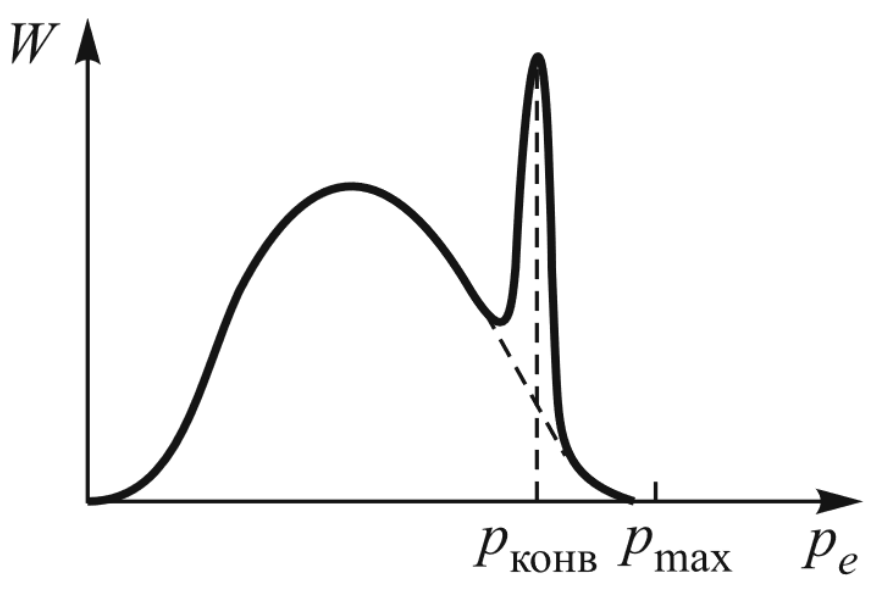
\includegraphics[width=0.6\linewidth]{pic1}
			\caption{Форма спектра $\beta$-частиц при разрешенных переходах}
		\end{figure}
		\section{Экспериментальная установка}
		Энергия определяется с помощью $\beta$-спектрометров. В работе используется магнитный спектрометр с короткой линзой.
		\begin{figure}[!htb]
			\centering
			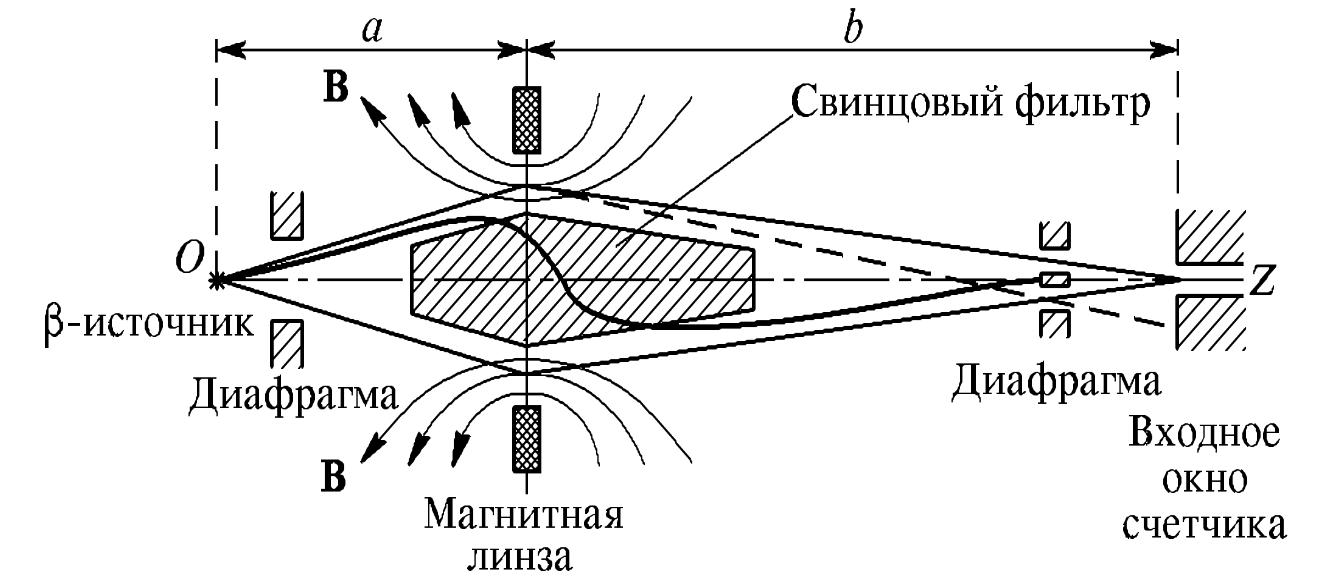
\includegraphics[width=0.8\linewidth]{pic2}
			\caption{Схема $\beta$-спектрометра с короткой линзой}
		\end{figure}
		Как показывает расчет, для заряженных частиц тонкая катушка эквивалентна линзе:
		\begin{equation}
			\frac{1}{f} \simeq \frac{I^2}{p_e^2}
		\end{equation}
		При заданной силе тока на входное окно счетчика собираются электроны с определенным импульсом.
		\section{Ход работы}
		Снимем точки $\beta$-спектра. Фоновое излучение равно $N_b = 0.8098$. C учетом этого пересчитаем число частиц, зарегистрированных счетчиком.
		\begin{table}[!htb]
			\centering
			\caption{Значения, полученные в ходе эксперимента}
			\label{tab:experiment}
			\begin{tabular}{|c|c|c|c|c|c|c|}
				\hline
				\# & $J$, A & $N$ & $N-N_b$ & $p$, кэВ/с & $T$, кэВ & mkFermi\\
				\hline
				1 & 0 & 0.88 & 0.0702 & 0. & 0 & 0 \\
 2 & 0.2 & 0.8 & -0.0098 & 49.2619 & 2.36901 & 0. \\
 3 & 0.4 & 0.84 & 0.0302 & 98.5238 & 9.41134 & 177.702 \\
 4 & 0.6 & 0.93 & 0.1202 & 147.786 & 20.9414 & 192.976 \\
 5 & 0.8 & 0.98 & 0.1702 & 197.048 & 36.6759 & 149.15 \\
 6 & 1 & 1.33 & 0.5202 & 246.31 & 56.2649 & 186.579 \\
 7 & 1.2 & 1.799 & 0.9892 & 295.571 & 79.325 & 195.726 \\
 8 & 1.4 & 2.459 & 1.6492 & 344.833 & 105.467 & 200.55 \\
 9 & 1.6 & 3.249 & 2.4392 & 394.095 & 134.316 & 199.628 \\
 10 & 1.8 & 3.719 & 2.9092 & 443.357 & 165.526 & 182.707 \\
 11 & 2 & 3.929 & 3.1192 & 492.619 & 198.785 & 161.531 \\
 12 & 2.2 & 4.219 & 3.4092 & 541.881 & 233.82 & 146.376 \\
 13 & 2.3 & 4.279 & 3.4692 & 566.512 & 251.927 & 138.134 \\
 14 & 2.4 & 4.489 & 3.6792 & 591.143 & 270.391 & 133.456 \\
 15 & 2.5 & 4.539 & 3.7292 & 615.774 & 289.187 & 126.379 \\
 16 & 2.6 & 4.199 & 3.3892 & 640.405 & 308.292 & 113.597 \\
 17 & 2.7 & 4.029 & 3.2192 & 665.036 & 327.686 & 104.618 \\
 18 & 2.8 & 4.239 & 3.4292 & 689.667 & 347.348 & 102.244 \\
 19 & 2.9 & 3.719 & 2.9092 & 714.298 & 367.261 & 89.3445 \\
 20 & 3 & 3.289 & 2.4792 & 738.929 & 387.408 & 78.3885 \\
 21 & 3.1 & 2.559 & 1.7492 & 763.559 & 407.774 & 62.6838 \\
 22 & 3.2 & 2.259 & 1.4492 & 788.19 & 428.343 & 54.4023 \\
 23 & 3.4 & 1.739 & 0.9292 & 837.452 & 470.045 & 39.7754 \\
 24 & 3.6 & 1.37 & 0.5602 & 886.714 & 512.418 & 28.3463 \\
 25 & 3.8 & 1.29 & 0.4802 & 935.976 & 555.383 & 24.1999 \\
 26 & 3.85 & 1.999 & 1.1892 & 948.292 & 566.209 & 37.3435 \\
 27 & 3.9 & 3.449 & 2.6392 & 960.607 & 577.066 & 54.5654 \\
 28 & 3.95 & 4.739 & 3.9292 & 972.923 & 587.954 & 65.3183 \\
 29 & 4 & 6.038 & 5.2282 & 985.238 & 598.872 & 73.9374 \\
 30 & 4.2 & 4.699 & 3.8892 & 1034.5 & 642.825 & 59.2699 \\
 31 & 4.25 & 4.659 & 3.8492 & 1046.82 & 653.88 & 57.9269 \\
 32 & 4.3 & 3.469 & 2.6592 & 1059.13 & 664.959 & 47.3098 \\
 33 & 4.35 & 2.159 & 1.3492 & 1071.45 & 676.064 & 33.1194 \\
 34 & 4.4 & 1.53 & 0.7202 & 1083.76 & 687.191 & 23.7862 \\
 35 & 4.5 & 0.8 & -0.0098 & 1108.39 & 709.515 & 0. \\
 36 & 4.6 & 0.43 & -0.3798 & 1133.02 & 731.926 & 0. \\
				\hline
			\end{tabular}
		\end{table}
		\par
		\newpage
		Для наглядности построим график зависимости N(J), полученный во время измерений.
		\begin{figure}[!htb]
			\centering
			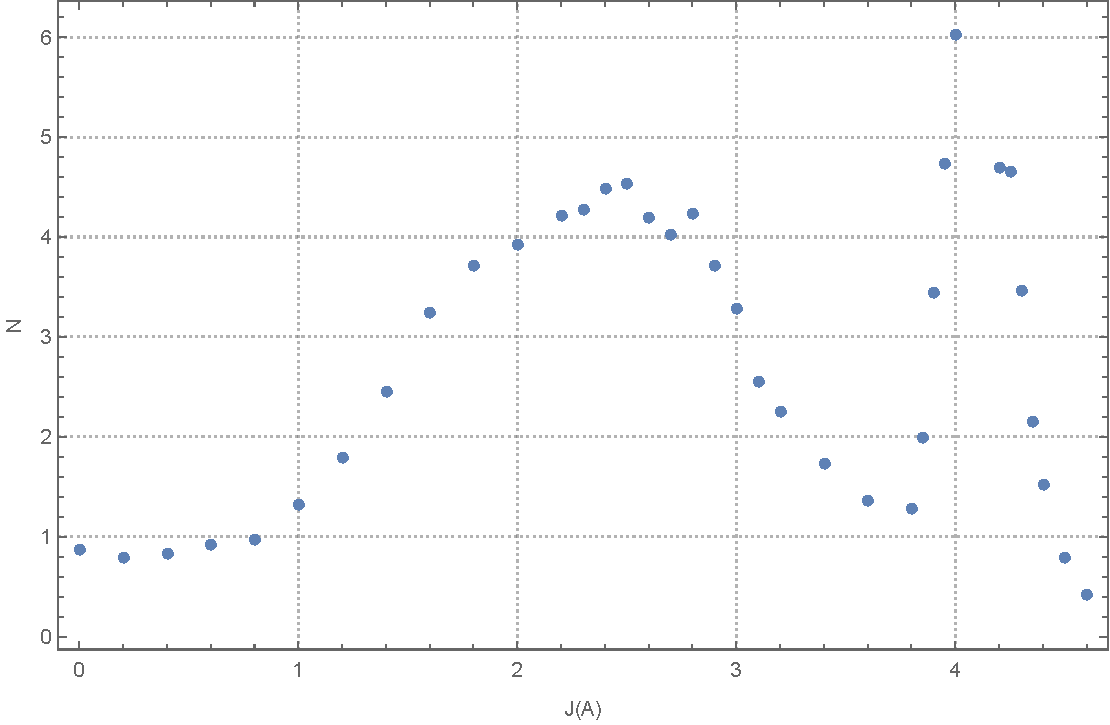
\includegraphics[width=\textwidth]{sourcePlot.pdf}
			\caption{Полученная зависимость $N(J)$}
		\end{figure}
		\par
		Знаем, что пик, наблюдаемый при силе тока около 4 А -- пик внутренней конверсии $^{137}$Cs. Его энергия соотвествует значению 634 кэВ. Согласно формуле (\ref{pToEConversion}), выражая $p$, получаем, что этот пик соотвествует значению импульса электрона $p_{\text{конв}}=1024.6476$ кэВ/$c$. Зависимость импульса электрона от тока имеет вид
		\begin{equation}
			\label{eq:currentToImpuls}
			p=kI.
		\end{equation}
		В качестве пика возьмем величину 4.16 А. Тогда $k=246.31$ кэВ/(А$c$). Таким образом c помощью формул (\ref{eq:currentToImpuls}) и (\ref{pToEConversion}) можем добавить значения импульса и энергии в таблицу \ref{tab:experiment}.\par
		Теперь можем посчитать значение последнего столбца таблицы \ref{tab:experiment} по формуле
		\begin{equation}
			F=\frac{\sqrt{n-n_b}\cdot 10^6}{p^{3/2}}.
		\end{equation}			
		Используя эту форумлу определим значения последнего столбца.\par
		Построим график Ферми-Кюри.
		\newpage
		\begin{figure}[!htb]
			\centering
			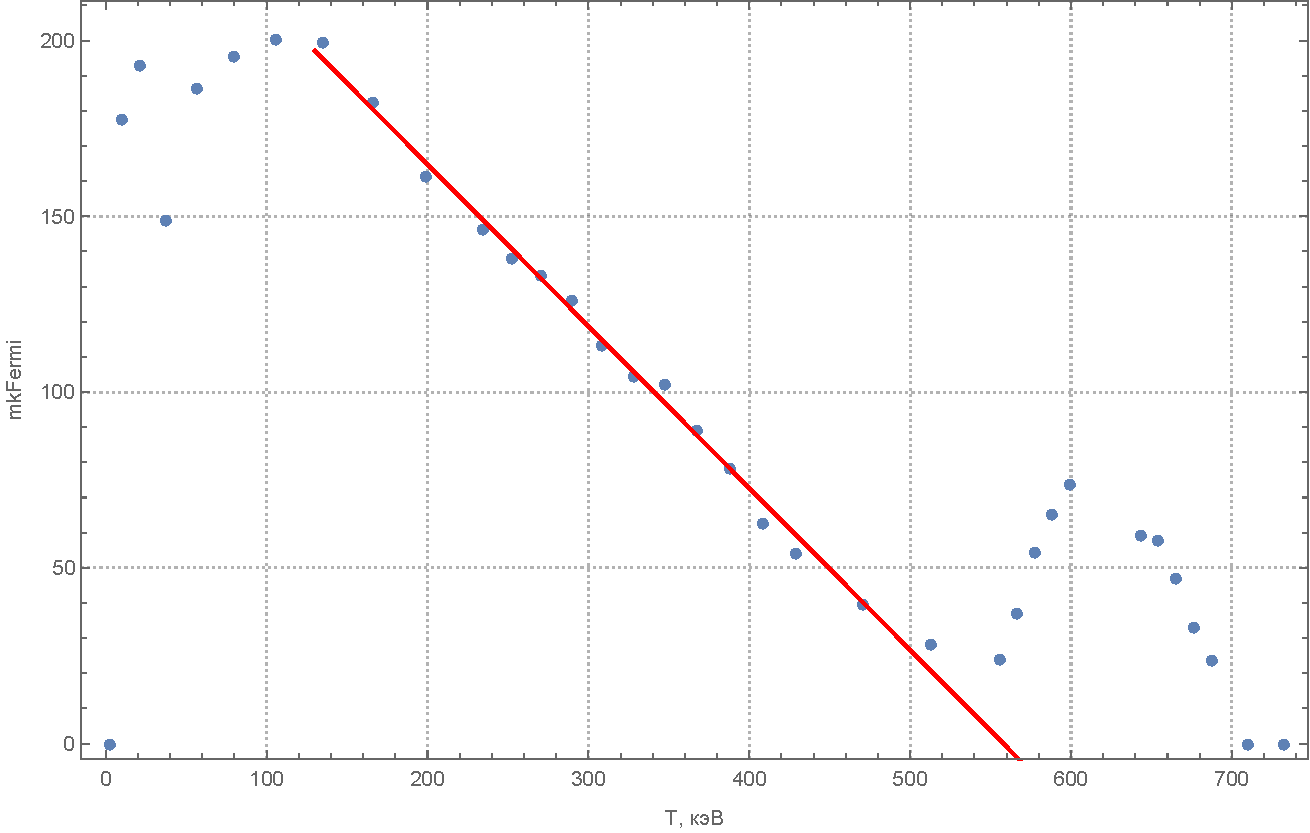
\includegraphics[width=\textwidth]{Fermi-Curie.pdf}
			\caption{График Ферми-Кюри}	
		\end{figure}
		\par
		Аппроксимируя участок графика получим уравнение прямой
		\begin{equation*}
			y=256.886-0.460457x
		\end{equation*}
		По точке пересечения графика с осью абсцисс определим максимальную энергию электронов в $\beta$-спектре. 
$E_{max} = 557.9$ кэВ.
\section{Вывод}
В проделанной работе было исследовано явление $\beta$-распада $^{137}Cs$. Выявлен <<полудискретный>> характер спектра: непрерывная часть обеспечивается за счет рождения двух частиц, дискретный пик --- рождение конверсионных электронов.
		Непрерывность спектра доказывает существование антинейтрино и его рождение в процессе $\beta^-$ распада. Также было выяснено существование конверсионных электронов --- частиц, испускаемых в результате перехода ядра на более низкий энергетический уровень. Их энергетический спектр является уже дискретным, т.к. их энергия строго привязана к энергиям жлектронных уровней в атоме.

\end{document}